\chapter{Planning}
\subsection{Gantt diagram}

A Gantt diagram~\ref{fig:gantt} is a representation of all the work hours, milestones and deadlines that is involved in the project. 

\begin{figure}[H]
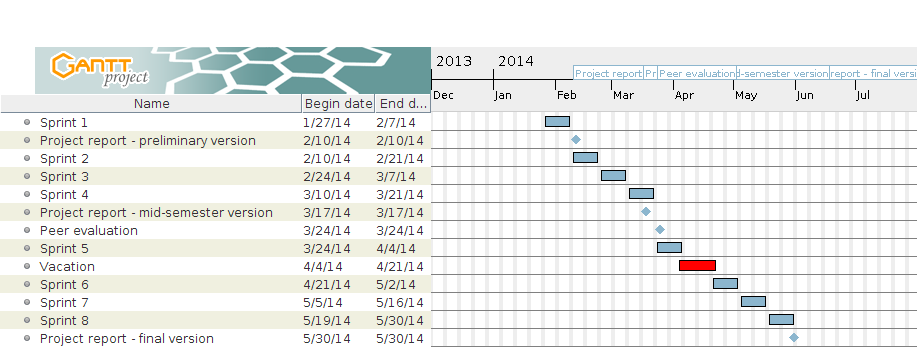
\includegraphics[width=\textwidth]{ch/planning/fig/gantt.png}
\caption{The Gantt diagram with sprints and milestones.}
\label{fig:gantt}
\end{figure}



\newpage
\input ch/planning/sec/wbs.tex
\newpage
\input ch/planning/sec/scrum.tex
\newpage
\input ch/planning/sec/risk.tex
\input ch/planning/sec/architecture.tex